%%%%%%%%%%%%%%%%%%%%%%%%%%%%%%%%%%%%%%%%%%%%%%%%%%%%%%%%%%%%%%%%%%%%%%%%%%%%%%%
%%                                                                           %%
%%   Dr Derek Harter                                                         %%
%%   Profesor, Department of Computer Science                                %% 
%%   Texas A&M University - Commerce, USA                                    %%
%%                                                                           %%
%%%%%%%%%%%%%%%%%%%%%%%%%%%%%%%%%%%%%%%%%%%%%%%%%%%%%%%%%%%%%%%%%%%%%%%%%%%%%%%
%%%%     SETTING STARTS - DO NOT CHANGE Unless your TeX setting require so   %%
%%%%%%%%%%%%%%%%%%%%%%%%%%%%%%%%%%%%%%%%%%%%%%%%%%%%%%%%%%%%%%%%%%%%%%%%%%%%%%%
%%----------------------------------------------------------------------------------
% DO NOT Change this. It is the required setting letterpaper page, 11pt, onside print, book style
%%----------------------------------------------------------------------------------
\documentclass[letterpaper,11pt,oneside]{book}

%%-------------------------------------
%% Page margin settings - % half inch margin all sides (recommended)
%%-------------------------------------
\usepackage[margin=1.2in]{geometry} 

%%-------------------------------------
%% Font settings - % CM San or Ariel (recommended)
%%-------------------------------------
% Switch the following two line off: to revert back to default LaTex font (NOT recommended)
\usepackage{amsfonts}
\renewcommand*\familydefault{\sfdefault}

%%-------------------------------------
%% Math/Definition/Theorem/Algorithm packages settings 
%%-------------------------------------
\usepackage[cmex10]{amsmath}
\usepackage{amssymb}
\usepackage{amsthm}
\newtheorem{mydef}{Definition}
\newtheorem{mytherm}{Theorem}

%%-------------------------------------
%% Algorithms/Code Listing environment settings  - 
%% Please do not change these settings
%%-------------------------------------
\usepackage{algorithm}
\usepackage{algpseudocode}
\renewcommand{\algorithmicrequire}{\textbf{Input:}}
\renewcommand{\algorithmicensure}{\textbf{Output:}}
\usepackage[utf8]{inputenc}
\usepackage{listings}
\usepackage{xcolor}
\definecolor{codegreen}{rgb}{0,0.6,0.1}
\definecolor{codegray}{rgb}{0.5,0.5,0.5}
\definecolor{codeblue}{rgb}{0.10,0.00,1.00}
\definecolor{codepurple}{rgb}{0.58,0,0.82}
\definecolor{backcolour}{rgb}{1.0,1.0,1.0}

\lstdefinestyle{mystyle}{
    backgroundcolor=\color{backcolour},   
    commentstyle=\color{codegreen},
    keywordstyle=\color{codeblue},
    numberstyle=\tiny\color{codegray},
    stringstyle=\color{codepurple},
    basicstyle=\ttfamily\footnotesize,
    breakatwhitespace=false,         
    breaklines=true,                 
    captionpos=b,                        
    keepspaces=true,                 
    numbers=left,                    
    numbersep=5pt,                  
    showspaces=false,                
    showstringspaces=false,
    showtabs=false,                  
    tabsize=2,
    frame=none
}
\lstset{style=mystyle}

%%-------------------------------------
%% Graphics/Figures environment settings
%%-------------------------------------
\usepackage{graphicx}
\usepackage{subfigure}
\usepackage{caption}
\usepackage{lipsum}

%%-------------------------------------
%% Table environment settings
%%-------------------------------------
\usepackage{multirow}
\usepackage{rotating}
\usepackage{makecell}
\usepackage{booktabs}
%\usepackage{longtable,booktabs}

%%-------------------------------------
%% List of Abbreviations settings
%%-------------------------------------
\usepackage{enumitem}
\newlist{abbrv}{itemize}{1}
\setlist[abbrv,1]{label=,labelwidth=1in,align=parleft,itemsep=0.1\baselineskip,leftmargin=!}

%%-------------------------------------
%% Bibliography/References settings   - Harvard Style was used in this report
%%-------------------------------------
\usepackage[hidelinks]{hyperref}
\usepackage[comma,authoryear]{natbib}
\renewcommand{\bibname}{References} % DO NOT remove or switch of 

%%-------------------------------------
%% Appendix settings     
%%-------------------------------------
\usepackage[toc]{appendix}
%%%%%%%%%%%%%%%%%%%%%%%%%%%%%%%%%%%%%%%%%%%%%%%%%%%%%%%%%%%%%%%%%%%%%%%%%%%%%%%%%%%%%%%
%%%%                     SETTING ENDS                                            %%%%%%
%%%%%%%%%%%%%%%%%%%%%%%%%%%%%%%%%%%%%%%%%%%%%%%%%%%%%%%%%%%%%%%%%%%%%%%%%%%%%%%%%%%%%%%
\begin{document}

    \captionsetup[figure]{margin=1.5cm,font=small,name={Figure},labelsep=colon}
    \captionsetup[table]{margin=1.5cm,font=small,name={Table},labelsep=colon}
    \SetLipsumDefault{1}
    
    \frontmatter
    
    \begin{titlepage}      
        \begin{center}
            
\includegraphics[width=3cm]{figures/tamuc-logo.png}\\[0.5cm]
            {\LARGE Texas A\&M University - Commerce\\[0.5cm]
            Department of Computer Science}\\[2cm]
			%{\color{blue} \rule{\textwidth}{1pt}}
			
			% -------------------------------
			% You need to edit some details here
			% -------------------------------  
            \linespread{1.2}\huge {
                %%%%%%%%%%%%%%%%%%%%%%%%%%%%
                %TODO: 1 TITLE of Your PROJECT 
                %%%%%%%%%%%%%%%%%%%%%%%%%%%%
                % chnage the following line                
                Comparison of SVM and Random Forests for Heart Disease Risk Prediction
            
            }
            \linespread{1}~\\[2cm]
			%{\color{blue} \rule{\textwidth}{1pt}}
            {\Large 
                %%%%%%%%%%%%%%%%%%%%%%%%%%%%
                %TODO: 2 YOUR NAME
                %%%%%%%%%%%%%%%%%%%%%%%%%%%%             
                % chnage the following line
                Lakshmi Chandana Narra
                % change end             
            }\\[1cm] 
            

            {\large 
                %%%%%%%%%%%%%%%%%%%%%%%%%%%%
                %TODO: 3 YOUR NAME Supervisor's name(s)
                %%%%%%%%%%%%%%%%%%%%%%%%%%%%             
                % change the following line                
                \emph{Supervisor:} Derek Harter, Ph.D.}\\[1cm] % if applicable
            
    		% PLEASE DO NOT CHANGE THIS TEXT %
            \large A report submitted in partial fulfilment of the requirements of\\Texas A\&M University - Commerce for the degree of\\ Master of Science in \textit{Computer Science}\\[0.3cm] 
            \vfill
            
            
            \today % Please update this date you can use \date{April 2020} for fixed date
        \end{center}
    \end{titlepage}
    
    
    % -------------------------------------------------------------------
    % Declaration
    % -------------------------------------------------------------------
    \newpage
    \thispagestyle{empty}
    \chapter*{\Large Declaration}
    % PLEASE CHANGE THIS TEXT EXCEPT YOUR NAME%
    % -------------------------------
    %TODO: PLEASE ONLY UPDATE HERE -- PLEASE WRITE YOUR NAME %    
    % ------------------------------- 
    I,
    %%%%%%%%%%%%%%%%%%%%%%%
     Lakshmi Chandana Narra, % Mandatory part
    %%%%%%%%%%%%%%%%%%%%%%%
    of the Department of Computer Science, Texas A\&M University - Commerce, confirm that this is my own work and figures, tables, equations, code snippets, artworks, and illustrations in this report are original and have not been taken from any other person's work, except where the works of others have been explicitly acknowledged, quoted, and referenced. I understand that if failing to do so will be considered a case of plagiarism. Plagiarism is a form of academic misconduct and will be penalised accordingly. \\
    
    %% Please delete as appropriate. 
    \noindent
    %%%%%%%%%%%%%%%%%%%%%%%%%%%%%%%%%%%%%%%%%%%%%%% 
    %TODO 1 Consent for example copy -  we will use 
    I give consent to a copy of my report being shared with future students as an exemplar. \\
    
    \noindent
    %%%%%%%%%%%%%%%%%%%%%%%%%%%%%%%%%%%%%%%%%%%%%%% 
    %TODO 2 Consent to let the report to use use by library for public use
    I give consent for my work to be made available more widely to members of TAMUC and public with interest in teaching, learning and research. 
    %%%%%%%%%%%%%%%%%%%%%%%%%%%%%%%%%%%%%%%%%%%%%%%
    ~\\[1cm]
    \begin{flushright}
	%------------------------------ 
	% change the following line
    %TODO: PLEASE UPDATE  Your Name  -------------------------------%
	Lakshmi Chandana Narra % Please change it to your name
    
    \today
    \end{flushright}

     
    % -------------------------------------------------------------------
    % Abstract and Acknowledgement
    % -------------------------------------------------------------------
    
    %Two resources useful for abstract writing.
% Guidance of how to write an abstract/summary provided by Nature: https://cbs.umn.edu/sites/cbs.umn.edu/files/public/downloads/Annotated_Nature_abstract.pdf %https://writingcenter.gmu.edu/guides/writing-an-abstract
\chapter*{\center \Large  Abstract}
%%%%%%%%%%%%%%%%%%%%%%%%%%%%%%%%%%%%%%
% Replace all text with your text
%%%%%%%%%%%%%%%%%%%%%%%%%%%%%%%%%%%

In recent times, the global rise in cardiovascular diseases has become increasingly prevalent, influenced by evolving lifestyles and societal factors. Emphasizing the need for timely detection and ongoing monitoring, particularly in regions with limited medical resources. Utilizing a public health dataset on patient heart health, including information from medical procedures and ongoing patient monitoring, this research uniquely centers on the comparative analysis of SVM and Random Forests. Focused on these two algorithms, this research aligns with the evolving landscape of machine learning in healthcare, presenting a concentrated perspective on their potential contributions. The methodology involves training SVM and Random Forest models on the dataset, evaluating their performance using key accuracy metrics such as the confusion matrix, Accuracy, precision, and F1 score. The study anticipates achieving comparable accuracy between the models but aims to determine their relative strengths in precision, recall, and F1 scores. This research aims to provide insights into which algorithm may be better suited for addressing the challenges associated with cardiovascular health monitoring, taking into consideration all parameters assessed in the research conclusion.
\\

\noindent % Provide your key words
\\

\textbf{Keywords:} Machine Learning, Random Forest, Support Vector Machine, Cardiovascular disease , Healthcare

\vfill
\noindent



    % -------------------------------------------------------------------
	% Acknowledgement
	% -------------------------------------------------------------------
   
    \chapter*{\center \Large  Acknowledgements}
%%%% Update with your text %%%%%%%%%%%%%%%
An acknowledgements section is optional. You may like to acknowledge the support and help of your supervisor(s), friends, or any other person(s), department(s), institute(s), etc. If you have been provided specific facility from department/school acknowledged so.  

   
    
    % -------------------------------------------------------------------
    % Contents, list of figures, list of tables
    % -------------------------------------------------------------------
    
    \tableofcontents
    \listoffigures
    \listoftables
    \chapter*{List of Abbreviations}
\chaptermark{List of Abbreviations}
%%%%%%%%%%%%%%%%%%%%%%%%%%%%%%%%%%%
%%  Enter your list of Abbreviation and Symbols in this file
%%%%%%%%%%%%%%%%%%%%%%%%%%%%%%%%%%%
\begin{abbrv}
    
    \item[SVM]			Support 
    Vector Machine
    \item[RF]			Random 
    Forest
\end{abbrv}
 %  Enter your list of Abbreviation and Symbols in this file
    
    %%%%%%%%%%%%%%%%%%%%%%%%%%%%%%%%%%%%%%%%%%%%%%%%%%%%%%%%%%%%%%%%%%%%%%%%
    %%                                                                    %%  
    %%  Main chapters and sections of your project                        %%  
    %%  Everything from here on needs updates in your own words and works %%
    %%                                                                    %%
    %%%%%%%%%%%%%%%%%%%%%%%%%%%%%%%%%%%%%%%%%%%%%%%%%%%%%%%%%%%%%%%%%%%%%%%%
    \mainmatter
    % Read for preparation of document in LaTex 
     
    
    \chapter{Introduction}
\label{ch:into} % This how you label a chapter and the key (e.g., ch:into) will be used to refer this chapter ``Introduction'' later in the report. 
% the key ``ch:into'' can be used with command \ref{ch:intor} to refere this Chapter.

Cardiovascular diseases represent a formidable global health challenge, with their prevalence 
escalating and ranking among the primary causes of morbidity and mortality. The pressing 
concern is the need for robust predictive models to address the increasing burden of heart 
diseases, enabling early detection and effective risk mitigation strategies.
\\


  

%%%%%%%%%%%%%%%%%%%%%%%%%%%%%%%%%%%%%%%%%%%%%%%%%%%%%%%%%%%%%%%%%%%%%%%%%%%%%%%%%%%
\section{Background}
\label{sec:into_back}

This research project delves into the development and 
evaluation of predictive models for heart disease using machine learning algorithms, 
specifically focusing on Support Vector Machines (SVM) and Random Forests(RF). The scope encompasses 
a comprehensive analysis of these algorithms, exploring their capabilities and limitations in 
accurately predicting the risk of cardiovascular events. The context of the project revolves 
around leveraging a diverse dataset derived from various medical procedures and continuous 
patient monitoring to enhance our understanding of heart disease prediction.
\\

The background of this study lies in the evolving landscape of lifestyle, dietary habits, and 
healthcare dynamics that contribute to the increasing prevalence of cardiovascular diseases. 
The significance of early detection and continuous monitoring underscores the importance of 
advanced \cite{toma2023predictive}predictive modeling techniques. Against this backdrop, the research aims to contribute 
to the field of cardiovascular health by providing insights into the efficacy of SVM and Random 
Forest algorithms.

In \cite{kumari2023comparative}  a comparative study on classification methods namely
Ripper, Decision Tree, Artificial neural networks and Support
Vector Machine are analyzed on cardiovascular disease
dataset.

In \cite{yanwei2007combination}it is establishes that a number of factors have been
shown to increase the risk of developing heart disease. Some
of these family history, high levels of LDL bad cholesterol,
Family history of cardiovascular disease, High levels of LDL
(bad) cholesterol, Low level of HDL (good) cholesterol,
Hypertension, High fat diet, Lack of regular exercise,
Obesity.

\\



In summary, the investigated problem centers on the escalating prevalence of cardiovascular diseases, and the project's scope involves the development and evaluation of predictive models using SVM and Random Forest. The background highlights the contextual relevance of advanced predictive modeling in addressing the challenges posed by heart diseases in the contemporary healthcare landscape.


%%%%%%%%%%%%%%%%%%%%%%%%%%%%%%%%%%%%%%%%%%%%%%%%%%%%%%%%%%%%%%%%%%%%%%%%%%%%%%%%%%%
\section{Problem statement}
\label{sec:intro_prob_art}

The research question guiding this study is: "How do Support Vector Machines (SVM) and Random Forest algorithms differ in terms of accuracy, efficiency, and interpretability when predicting the risk of heart disease?"

The prevalence of cardiovascular diseases is increasing globally, necessitating accurate and efficient predictive models for early detection and intervention. However, selecting the most suitable algorithm for this task poses a challenge. This research aims to compare and examine the differential performance of SVM and Random Forests in predicting the risk of heart disease. By leveraging real-world data\cite{lapp-heart-disease-dataset-1988} on patient heart health, the study seeks to uncover the unique strengths and limitations of each algorithm. Through this investigation, the research aims to provide insights into selecting appropriate machine learning algorithms to enhance cardiovascular health monitoring and decision-making in clinical practice.



%%%%%%%%%%%%%%%%%%%%%%%%%%%%%%%%%%%%%%%%%%%%%%%%%%%%%%%%%%%%%%%%%%%%%%%%%%%%%%%%%%%
\section{Aims and objectives}
\label{sec:intro_aims_obj}




This research project's main goal is to evaluate and contrast the effectiveness of Random Forest and Support Vector Machines (SVM) algorithms in relation to risk assessments for heart disease. The main objective is to advance predictive modeling methods for accurate assessment and early identification of cardiac disease.

\


\begin{itemize}
  \item Analyze and clean the Kaggle heart disease dataset, preparing it for building predictive models.
  \item Develop a Support Vector Machine (SVM) classifier and train it on the preprocessed heart disease data.
  \item Build a Random Forest (RF) classifier and train it on the same preprocessed data.
  \item Conduct parameter tuning to maximize the performance of both models, focusing on recall, precision, and/or F1 scores.
  \item Compare the recall, precision, and  accuracy of the resulting SVM and RF models.
  \item Evaluate and interpret the performance of SVM and RF models in predicting heart disease risk.
  \item Identify the strengths and weaknesses of each model in the context of cardiovascular health monitoring.
  \item Draw conclusions and provide recommendations for selecting the most suitable machine learning algorithm for heart disease risk analysis.
\end{itemize}



%%%%%%%%%%%%%%%%%%%%%%%%%%%%%%%%%%%%%%%%%%%%%%%%%%%%%%%%%%%%%%%%%%%%%%%%%%%%%%%%%%%
\section{Solution approach}
\label{sec:intro_sol} % label of Org section
\textbf{Data Preparation:} Prepare the Kaggle heart disease dataset for the construction of predictive models by analyzing and cleaning it.
\\
\textbf{Model Development:} Using the preprocessed cardiac disease data, create an SVM classifier and train it. Using the same preprocessed data, create and train a Random Forest (RF) classifier.
\\
\textbf{Model Assessment:} Optimize both models' performance by fine-tuning their parameters with an emphasis on recall, precision, and/or F1 scores.

Print the assessment measures for each of the two models:
\begin{itemize}
    \item Metrics for the SVM Model: F1 Score, Accuracy, Precision, Recall.
    \item Metrics for the Random Forest Model: F1 Score, Accuracy, Precision, Recall.
\end{itemize}

Print the two models' confusion matrices.
\\
\textbf{Model Comparison:} Based on the evaluation metrics and confusion matrices, compare the SVM and Random Forest models' performances. Analyze and assess how well the RF and SVM models predict the risk of heart disease. Determine each model's advantages and disadvantages in relation to cardiovascular health monitoring.
\\
\textbf{Concluding remarks and suggestions:}
\begin{itemize}
    \item Make inferences from the performance comparison.
    \item Make suggestions on which machine learning algorithm would be best for analyzing the risk of heart disease.
\end{itemize}

The measures used to answer the research topic of comparing and contrasting the efficiency of Random Forest and SVM algorithms for heart disease risk assessments are described in this solution methodology. Data preparation, model construction, assessment, comparison, and conclusion are all included, giving your research a thorough approach.



%%%%%%%%%%%%%%%%%%%%%%%%%%%%%%%%%%%%%%%%%%%%%%%%%%%%%%%%%%%%%%%%%%%%%%%%%%%%%%%%%%%
\section{Summary of contributions and achievements} %  use this section 
\label{sec:intro_sum_results} % label of summary of results



%%%%%%%%%%%%%%%%%%%%%%%%%%%%%%%%%%%%%%%%%%%%%%%%%%%%%%%%%%%%%%%%%%%%%%%%%%%%%%%%%%%



    \chapter{Literature Review}
\label{ch:lit_rev} %Label of the chapter lit rev. The key ``ch:lit_rev'' can be used with command \ref{ch:lit_rev} to refer this Chapter.

This section explores the efficacy of machine learning (ML) in the prediction of cardiovascular disease (CVD). ML learns from data and experience through training, enabling it to be applied to various tasks based on specific algorithms. This flexibility enables ML algorithms to analyze complex datasets and predict CVD risk.

A review of existing literature is also done to investigate previously published studies in the area. This review  helps to contextualize the current findings. The literature review for this study will look at earlier research on machine learning (ML) in disease prediction, including various algorithms and their effectiveness. This understanding is crucial for developing accurate and effective predictive models for CVD.

% PLEAE CHANGE THE TITLE of this section
\section{Review of State-of-the-art} 
% Note the use of \cite{} and \citep{}
Previous studies, such as that by \cite{seema2016predictive}, have focused on predicting chronic diseases by analyzing data from historical health records. They employed various techniques, including Naïve Bayes, Decision Trees, Support Vector Machines (SVM), and Artificial Neural Networks (ANN). Through a comparative study of these classifiers, the researchers evaluated their performance in terms of accuracy. Their findings indicate that SVM achieved the highest accuracy rate overall, while Naïve Bayes showed the best performance in predicting diabetes.

\cite{shetty2016different} proposed the development of a predictive system for diagnosing heart disease using patient medical datasets. They considered 13 risk factors as input attributes for building the system. The data from the dataset was analyzed, and processes such as data cleaning and data integration were performed.
\

\cite{pal2021prediction}In this study, the researchers implemented the random forest data mining algorithm to predict heart disease. Their experimental results showed a sensitivity of 90.6, specificity of 82.7, and an overall accuracy of 86.9 for heart disease prediction. The proposed system achieved a classification accuracy of 86.9 and a diagnosis rate of 93.3 using the random forest algorithm. The researchers suggest that the system could also be used for predicting other diseases by applying different machine learning algorithms such as Naïve Bayes, decision tree, K-NN, linear regression, and fuzzy logic to improve accuracy. They also propose the use of cloud computing technology to manage large volumes of patient data.

\section{Machine Learning : SVM and Random Forest }

\subsection{Machine Learning}

In the realm of artificial intelligence, machine learning is dedicated to developing statistical models and algorithms that enhance a computer's performance in specific tasks without the need for explicit programming. It revolves around utilizing statistical models and algorithms to execute tasks without direct instructions, relying heavily on pattern recognition and prediction.

\subsection{Support Vector Machine}

A supervised machine learning approach called Support Vector Machine (SVM) is commonly used for classification problems, while it can also be used for regression tasks. The way SVM works is that it finds the hyperplane in the input data set that best divides different classes. The margin, or the distance between the hyperplane and the nearest data point from each class also known as the support vectors is optimized when choosing this particular hyperplane. Because SVM uses a small amount of memory and performs well in high-dimensional spaces, it can be used to datasets with a large number of features.

\subsection{Random Forest}

In order to create the class that represents the mean prediction (for regression) or the mode of the classes (for classification), Random Forest is an ensemble learning technique that creates many decision trees during training. Each tree in a Random Forest is trained using a subset of the training set, and the ultimate prediction can be determined by polling (for classification) or by averaging the predictions of all the trees (for regression). High accuracy, scalability, and the capacity to handle big datasets with high dimensionality are attributes of Random Forest.






% A possible section of you chapter
\section{Critique of the review} % Use this section title or choose a betterone
The literature review offers insightful information about the application of machine learning algorithms more especially, SVM and Random Forest for the diagnosis and prognosis of cardiac disease.\cite{seema2016predictive}revealed how SVM may be used to achieve high overall accuracy, while Naive Bayes showed encouraging findings in terms of diabetes prediction. This implies that SVM would work well for our research on the identification of heart disease, especially given its ability to hande high-dimensional data.

 ~\\
\cite{shetty2016different}highlighted the significance of feature selection in machine learning models by proposing a prediction strategy for diagnosing heart disease based on 13 risk variables. This can be a useful case study for our work, highlighting the necessity of selecting relevant characteristics with consideration in order to increase the accuracy of our model.
~\\
\

\cite{pal2021prediction} achieved a high sensitivity, specificity, and overall accuracy in their implementation of Random Forest for heart disease prediction. Their methodology demonstrates how ensemble approaches can enhance prediction performance, and we can take this into account when comparing Random Forest and SVM in our own study.

\








% Pleae use this section
\section{Summary} 
Overall, the reviewed studies provide a solid foundation and examples for our research on comparing SVM and Random Forest for heart disease detection. We can leverage their methodologies and findings to design our experiments, select appropriate features, and evaluate the performance of the algorithms effectively.% https://guides.library.bloomu.edu/litreview
    % replace all text with your own text.
% in this template few examples are mention
\chapter{Methodology}
\label{ch:method} % Label for method chapter


\section{Dataset Description}

The Kaggle heart disease dataset\cite{lapp-heart-disease-dataset-1988}, which has 1025 samples with 14 attributes each, was used in this investigation. The dataset includes a number of clinical characteristics that are frequently used to determine whether a patient has cardiac disease. Each sample has the following characteristics and represents a patient:

\begin{enumerate}
    \item Age (\textit{age}): The age of the patient in years.
    \item Sex (\textit{sex}): The gender of the patient (1 = male, 0 = female).
    \item Chest Pain Type (\textit{cp}): The type of chest pain experienced by the patient, categorized into four types: typical angina (1), atypical angina (2), non-anginal pain (3), and asymptomatic (4).
    \item Resting Blood Pressure (\textit{trestbps}): The resting blood pressure of the patient in mm Hg.
    \item Serum Cholesterol (\textit{chol}): The serum cholesterol level of the patient in mg/dl.
    \item Fasting Blood Sugar (\textit{fbs}): The fasting blood sugar level of the patient, where 1 indicates a fasting blood sugar level greater than 120 mg/dl and 0 indicates a level less than or equal to 120 mg/dl.
    \item Resting Electrocardiographic Results (\textit{restecg}): The resting electrocardiographic results of the patient, categorized into three types: normal (0), having ST-T wave abnormality (1), and showing probable or definite left ventricular hypertrophy (2).
    \item Maximum Heart Rate Achieved (\textit{thalach}): The maximum heart rate achieved by the patient.
    \item Exercise-Induced Angina (\textit{exang}): Whether the patient experienced exercise-induced angina (1 = yes, 0 = no).
    \item ST Depression Induced by Exercise Relative to Rest (\textit{oldpeak}): The ST depression induced by exercise relative to rest.
    \item Slope of the Peak Exercise ST Segment (\textit{slope}): The slope of the peak exercise ST segment, categorized into three types: upsloping (1), flat (2), and downsloping (3).
    \item Number of Major Vessels Colored by Fluoroscopy (\textit{ca}): The number of major vessels colored by fluoroscopy, ranging from 0 to 3.
    \item Thalassemia (\textit{thal}): The thalassemia status of the patient, categorized into three types: normal (3), fixed defect (6), and reversible defect (7).
    \item Target (\textit{target}): The presence of heart disease in the patient, where 1 indicates the presence of heart disease and 0 indicates the absence of heart disease.
\end{enumerate}
\subsection{Target Variable}
The target variable, \textit{target}, indicates the presence of heart disease and is binary, where 1 represents disease present and 0 represents disease not present.

\subsection{Data Types}
The dataset consists of the following features with their respective data types:
\begin{itemize}
    \item \textbf{age}: integer
    \item \textbf{sex}: integer
    \item \textbf{cp}: integer
    \item \textbf{trestbps}: integer
    \item \textbf{chol}: integer
    \item \textbf{fbs}: integer
    \item \textbf{restecg}: integer
    \item \textbf{thalach}: integer
    \item \textbf{exang}: integer
    \item \textbf{oldpeak}: float
    \item \textbf{slope}: integer
    \item \textbf{ca}: integer
    \item \textbf{thal}: integer
    \item \textbf{target}: integer
\end{itemize}




\begin{figure}
    \centering
    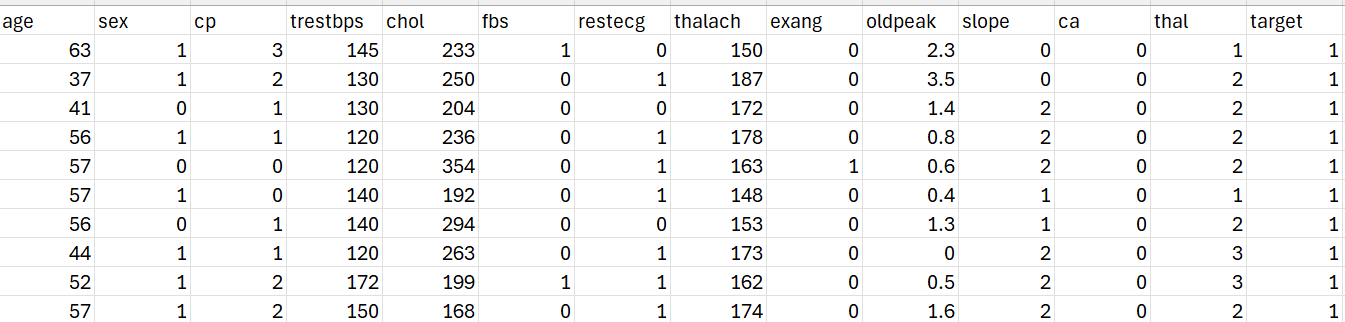
\includegraphics[width=1.0\textwidth]{figures/Datasettop10patients.png}
    \caption{Top 10 patient data from dataset}
    \label{fig:example}
\end{figure}
\section{Software Used}
The implementation and comparison of SVM and Random Forest models were performed using Python along with the following libraries:
\begin{itemize}
    \item \textbf{Python}: Python programming language was used as the primary language for coding the models.
    \item \textbf{pandas}: The pandas library was utilized for data manipulation and analysis, including reading the dataset, creating dataframes, and structuring the data.
    \item \textbf{scikit-learn (sklearn)}: The scikit-learn library was used for implementing the SVM and Random Forest algorithms, as well as for data preprocessing, model training, and evaluation.
\end{itemize}
These libraries provided the necessary tools and functions to effectively implement and compare the models, ensuring a robust and efficient analysis of the dataset.

\section{Data preparation and cleaning}
As an initial step for preparing and cleaning data in this study, a dataset comprising 1025 samples is read from a CSV file and transformed into a table using Python's pandas library. This procedure involves loading the dataset, associating the columns with their corresponding values, and constructing a table containing the samples. This process is crucial for structuring the data in an organized manner, which will simplify subsequent tasks such as data cleaning, managing missing values, and preparing the data for training and testing the SVM and Random Forest models.
\subsection{Dataset Loading and Data Type Definition}To prepare the data for analysis, I first categorized each column based on its data type. Subsequently, I imported the dataset from a CSV file into a Pandas DataFrame. This step was crucial for organizing and analyzing the data efficiently.
\begin{figure}
    \centering
    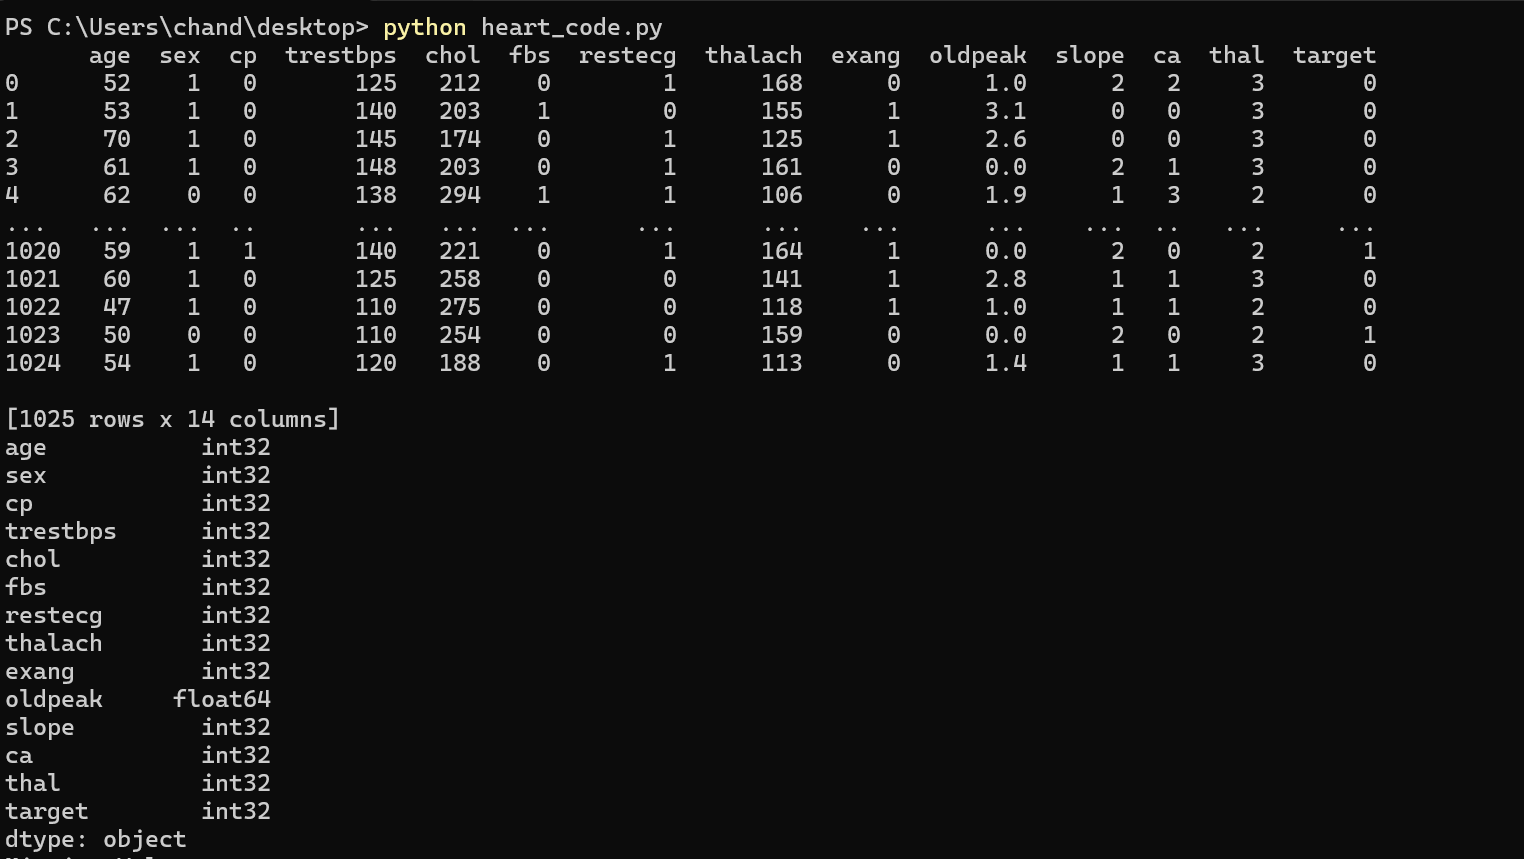
\includegraphics[width=1.0\textwidth]{figures/loaddata.png}
    \caption{Load data and data type definition}
    \label{fig:example}
\end{figure}
Table~\ref{tab:algo_temp} may suit you the best. 
\begin{table}[ht!]
    \centering
    \caption{Example of an algorithm analysis type report structure}
    \label{tab:algo_temp}
    \begin{tabular}{lll}     
        \toprule                   
        Chapter 1 & Introduction  &    \\        
        Chapter 2 & Literature Review  &    \\                
        Chapter 3 & Methodology   &    \\
        &               & Algorithms descriptions  \\
        &               & Implementations   \\
        &               & Experiments design   \\
        Chapter 4 & Results       &  \\
        Chapter 5 & Discussion and Analysis  &    \\
        Chapter 6 & Conclusion and Future Work  &    \\        
        Chapter 7 & Reflection  &    \\          
        \bottomrule
    \end{tabular}
\end{table}


\subsection{Example of a science lab-type main text structure}
If you are doing a science lab experiment type of project, you may use the  methodology section suggested in Table~\ref{tab:lab_temp}. In this kind of project, you may refer to the ``Methodology'' section as ``Materials and Methods.''
\begin{table}[ht!]
    \centering
    \caption{Example of a science lab experiment-type report structure}
    \label{tab:lab_temp}
    \begin{tabular}{lll}     
        \toprule                   
        Chapter 1 & Introduction  &    \\        
        Chapter 2 & Literature Review  &    \\                
        Chapter 3 & Materials and Methods   &    \\
        &               & Problems (tasks) description  \\
        &               & Materials \\        
        &               & Procedures  \\                
        &               & Implementations   \\
        &               & Experiment set-up   \\
        Chapter 4 & Results       &  \\
        Chapter 5 & Discussion and Analysis  &    \\
        Chapter 6 & Conclusion and Future Work  &    \\        
        Chapter 7 & Reflection  &    \\          
        \bottomrule
    \end{tabular}
\end{table}

\section{Example of an Equation in \LaTeX}
Eq.~\ref{eq:eq_example} [note that this is an example of an equation's in-text citation] is an example of an equation in \LaTeX. In Eq.~\eqref{eq:eq_example}, $ s $ is the mean of elements $ x_i \in \mathbf{x} $: 

\begin{equation}
\label{eq:eq_example} % label used to refer the eq in text
s = \frac{1}{N} \sum_{i = 1}^{N} x_i. 
\end{equation}

Have you noticed that all the variables of the equation are defined using the \textbf{in-text} maths command \$.\$, and Eq.~\eqref{eq:eq_example} is treated as a part of the sentence with proper punctuation? Always treat an equation or expression as a part of the sentence. 

\section{Example of a Figure in \LaTeX}
Figure~\ref{fig:chart_a} is an example of a figure in \LaTeX. For more details, check the link:

\href{https://en.wikibooks.org/wiki/LaTeX/Floats,_Figures_and_Captions}{wikibooks.org/wiki/LaTeX/Floats,\_Figures\_and\_Captions}.

\noindent
Keep your artwork (graphics, figures, illustrations) clean and readable. At least 300dpi is a good resolution of a PNG format artwork. However, an SVG format artwork saved as a PDF will produce the best quality graphics. There are numerous tools out there that can produce vector graphics and let you save that as an SVG file and/or as a PDF file. One example of such a tool is the ``Flow algorithm software''. Here is the link for that: \href{http://www.flowgorithm.org/download/}{flowgorithm.org}.
\begin{figure}[ht]
    \centering
    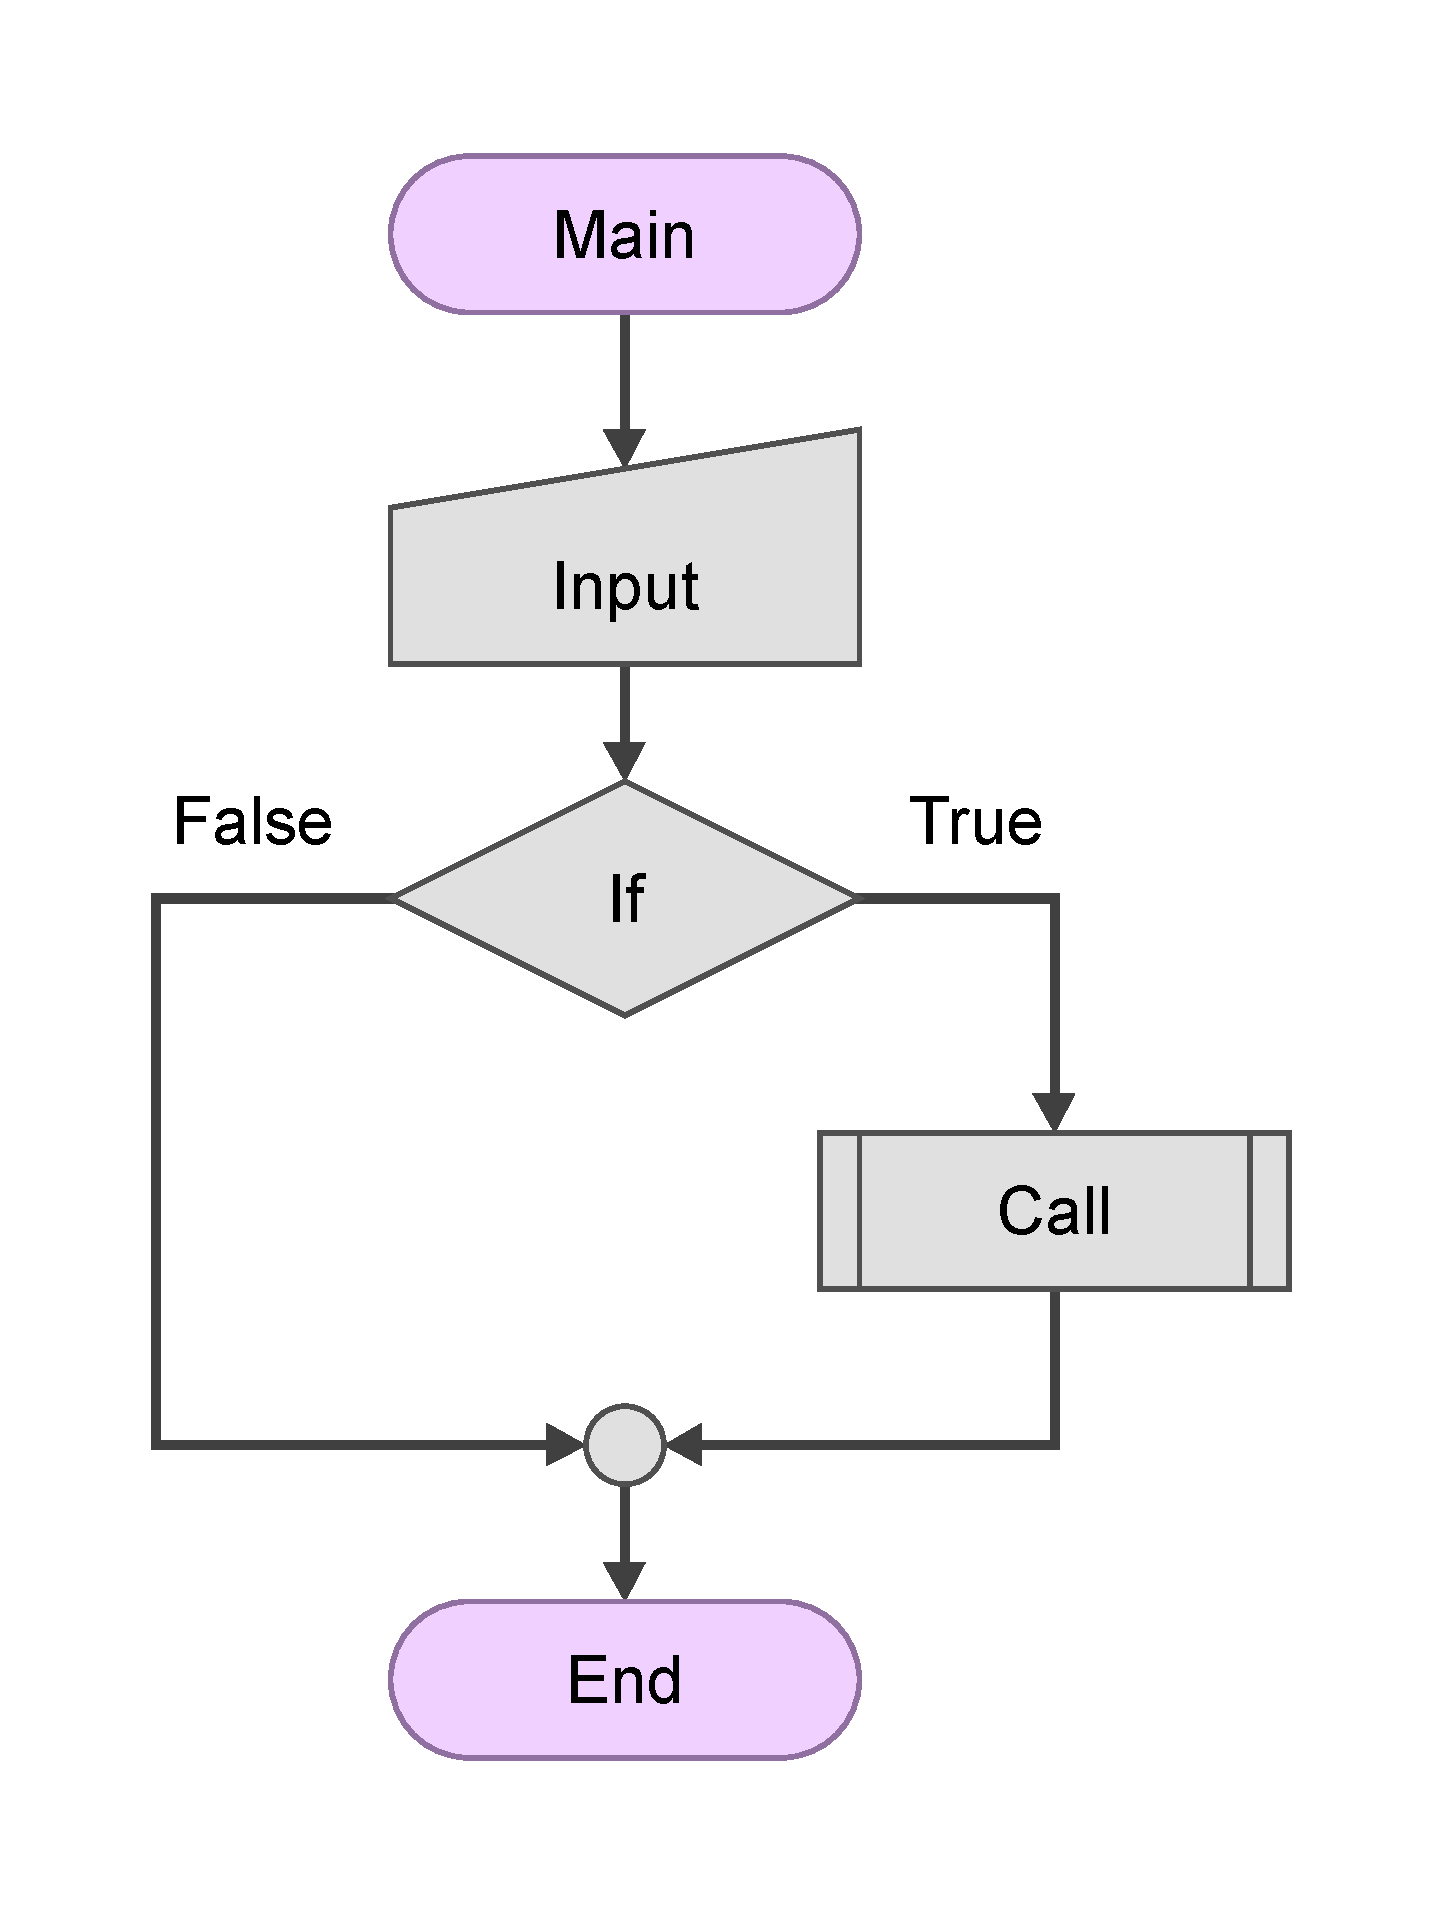
\includegraphics[scale=0.3]{figures/chart.pdf}
    \caption{Example figure in \LaTeX.}
    \label{fig:chart_a}
\end{figure}

\clearpage %  use command \clearpage when you want section or text to appear in the next page.

\section{Example of an algorithm in \LaTeX}
Algorithm~\ref{algo:algo_example} is a good example of an algorithm in \LaTeX.  
\begin{algorithm}
    \caption{Example caption: sum of all even numbers}
    \label{algo:algo_example}
    \begin{algorithmic}[1]
        \Require{$ \mathbf{x}  = x_1, x_2, \ldots, x_N$}
        \Ensure{$EvenSum$ (Sum of even numbers in $ \mathbf{x} $)}
        \Statex
        \Function{EvenSummation}{$\mathbf{x}$}
        \State {$EvenSum$ $\gets$ {$0$}}
        \State {$N$ $\gets$ {$length(\mathbf{x})$}}
        \For{$i \gets 1$ to $N$}                    
        \If{$ x_i\mod 2 == 0$}  \Comment check if a number is even?
        \State {$EvenSum$ $\gets$ {$EvenSum + x_i$}}
        \EndIf
        \EndFor
        \State \Return {$EvenSum$}
        \EndFunction
    \end{algorithmic}
\end{algorithm}
 
\section{Example of code snippet  in \LaTeX}

Code Listing~\ref{list:python_code_ex} is a good example of including a code snippet in a report. While using code snippets, take care of the following:
\begin{itemize}
    \item do not paste your entire code (implementation) or everything you have coded. Add code snippets only. 
    \item The algorithm shown in Algorithm~\ref{algo:algo_example} is usually preferred over code snippets in a technical/scientific report. 
    \item Make sure the entire code snippet or algorithm stays on a single page and does not overflow to another page(s).  
\end{itemize}

Here are three examples of code snippets for three different languages (Python, Java, and CPP) illustrated in Listings~\ref{list:python_code_ex}, \ref{list:java_code_ex}, and \ref{list:cpp_code_ex} respectively.  

\begin{lstlisting}[language=Python, caption={Code snippet in \LaTeX ~and  this is a Python code example}, label=list:python_code_ex]
import numpy as np

x  = [0, 1, 2, 3, 4, 5] # assign values to an array
evenSum = evenSummation(x) # call a function

def evenSummation(x):
    evenSum = 0
    n = len(x)
    for i in range(n):
        if np.mod(x[i],2) == 0: # check if a number is even?
            evenSum = evenSum + x[i]
    return evenSum
\end{lstlisting}

Here we used  the ``\textbackslash clearpage'' command and forced-out the second listing example onto the next page. 
\clearpage  %
\begin{lstlisting}[language=Java, caption={Code snippet in \LaTeX ~and  this is a Java code example}, label=list:java_code_ex]
public class EvenSum{ 
    public static int evenSummation(int[] x){
        int evenSum = 0;
        int n = x.length;
        for(int i = 0; i < n; i++){
            if(x[i]%2 == 0){ // check if a number is even?
                evenSum = evenSum + x[i];
            }
        }
        return evenSum;     
    }
    public static void main(String[] args){ 
        int[] x  = {0, 1, 2, 3, 4, 5}; // assign values to an array
        int evenSum = evenSummation(x);
        System.out.println(evenSum);
    } 
} 
\end{lstlisting}


\begin{lstlisting}[language=C, caption={Code snippet in \LaTeX ~and  this is a C/C++ code example}, label=list:cpp_code_ex]
int evenSummation(int x[]){
    int evenSum = 0;
    int n = sizeof(x);
    for(int i = 0; i < n; i++){
        if(x[i]%2 == 0){ // check if a number is even?
            evenSum = evenSum + x[i];
    	}
    }
    return evenSum;     
}

int main(){
    int x[]  = {0, 1, 2, 3, 4, 5}; // assign values to an array
    int evenSum = evenSummation(x);
    cout<<evenSum;
    return 0;
}
\end{lstlisting}



\section{Example of in-text citation style}
\subsection{Example of the equations and illustrations placement and reference in the text}
Make sure whenever you refer to the equations, tables, figures, algorithms,  and listings for the first time, they also appear (placed) somewhere on the same page or in the following page(s). Always make sure to refer to the equations, tables and figures used in the report. Do not leave them without an \textbf{in-text citation}. You can refer to equations, tables and figures more them once.

\subsection{Example of the equations and illustrations style}
Write \textbf{Eq.} with an uppercase ``Eq`` for an equation before using an equation number with (\textbackslash eqref\{.\}). Use ``Table'' to refer to a table, ``Figure'' to refer to a figure, ``Algorithm'' to refer to an algorithm and ``Listing'' to refer to listings (code snippets). Note that, we do not use the articles ``a,'' ``an,'' and ``the'' before the words Eq., Figure, Table, and Listing, but you may use an article for referring the words figure, table, etc. in general.

For example, the sentence ``A report structure is shown in \textbf{the} Table~\ref{tab:gen_template}'' should be written as ``A report structure is shown \textbf{in} Table~\ref{tab:gen_template}.'' 
 

\section{Summary}
Write a summary of this chapter.

~\\[5em]
\noindent
{\huge\textbf{Note:}} In the case of \textbf{software engineering} project a Chapter ``\textbf{Testing and Validation}'' should precede the ``Results'' chapter. See Section~\ref{subsec:se_chpters} for report organization of such project. 


    \chapter{Results}
\label{ch:results}
The results chapter tells a reader about your findings based on the methodology you have used to solve the investigated problem. For example: 
\begin{itemize}
    \item If your project aims to develop a software/web application, the results may be the developed software/system/performance of the system, etc., obtained using a relevant methodological approach in software engineering. 
    
    \item If your project aims to implement an algorithm for its analysis, the results may be the performance of the algorithm obtained using a relevant experiment design. 
    
    \item If your project aims to solve some problems/research questions over a collected dataset, the results may be the findings obtained using the applied tools/algorithms/etc. 
\end{itemize}
Arrange your results and findings in a logical sequence. 



\section{A section}

...

\clearpage
\section{Example of a Table in \LaTeX}
Table~\ref{tab:_ex_tab} is an example of a table created using the package \LaTeX  ``booktabs.'' do check the link: \href{https://en.wikibooks.org/wiki/LaTeX/Tables}{wikibooks.org/wiki/LaTeX/Tables} for more details. A table should be clean and readable. Unnecessary horizontal lines and vertical lines in tables make them unreadable and messy. The example in Table~\ref{tab:_ex_tab} uses a minimum number of liens (only necessary ones). Make sure that the top rule and bottom rule (top and bottom horizontal lines) of a table are present. 

\begin{table}[h!]
    \centering
    \caption{Example of a table in \LaTeX}
    \label{tab:_ex_tab}
    \begin{tabular}{llr}     
        \toprule
        \multicolumn{2}{c}{Bike} \\
        \cmidrule(r){1-2}
        Type    &  Color & Price (\pounds) \\
        \midrule
        Electric    & black   & 700   \\
        Hybrid      & blue    & 500   \\
        Road        & blue    & 300   \\
        Mountain    & red     & 300   \\
        Folding     & black   & 500   \\
        \bottomrule
    \end{tabular}
\end{table}

\section{Example of captions style}

\begin{itemize}
    \item The \textbf{caption of a Figure (artwork) goes below} the artwork (Figure/Graphics/illustration). See example artwork in Figure~\ref{fig:chart_a}. 
    \item  The \textbf{caption of a Table goes above} the table. See the example in Table~\ref{tab:_ex_tab}.
    \item  The \textbf{caption of an Algorithm goes above} the algorithm. See the example in Algorithm~\ref{algo:algo_example}.
    \item The \textbf{caption of a Listing goes below} the Listing  (Code snippet). See example listing in Listing~\ref{list:python_code_ex}. 
\end{itemize} 





\section{Summary}
Write a summary of this chapter.




    \chapter{Discussion and Analysis}
\label{ch:evaluation}

The performance comparison of the SVM and Random Forest models for the classification of heart disease is evaluated and examined in this chapter.


\section{Discussion on model performance}
The results show that the Random Forest model outperformed the SVM model in terms of training and testing accuracy, precision, recall, and F1 score. Specifically, the Random Forest model achieved a training accuracy of 91.29 and a testing accuracy of 80.33, while the SVM model achieved a training accuracy of 86.31 and a testing accuracy of 77.05.

The training and testing confusion matrices for the SVM model show that it correctly classified 85 and 23 cases of the negative class (no heart disease), respectively, and 123 and 24 cases of the positive class (heart disease), respectively. However, the SVM model misclassified 21 cases of the negative class as positive and 5 cases of the positive class as negative in the training and testing datasets, respectively.

On the other hand, the training and testing confusion matrices for the Random Forest model show that it correctly classified 95 and 89 cases of the negative class, respectively, and 123 and 24 cases of the positive class, respectively. However, the Random Forest model misclassified 11 cases of the negative class as positive and 1 case of the positive class as negative in the training dataset, and 5 cases of the negative class as positive in the testing dataset.



\section{Significance of the findings}
The key finding of this study is that the Random Forest model outperformed the SVM model in heart disease classification, achieving higher accuracy, precision, recall, and F1 score values for both training and testing datasets. This suggests that the Random Forest model is more effective in capturing the complex relationships between the features in the heart disease dataset.

The significance of this finding lies in the potential for Random Forest models to improve the accuracy of heart disease diagnosis, which can lead to better patient outcomes. The results of this study demonstrate that Random Forest models can achieve high accuracy rates in heart disease classification, even with imbalanced datasets. This is important because imbalanced datasets are common in medical applications, where the prevalence of certain diseases may be low.

\section{Limitations}  
There are several key limitations to this study that should be taken into account when interpreting the findings. First, the study used a relatively small dataset of 303 patients, which may limit the generalizability of the results to larger and more diverse populations. Second, the study did not consider the impact of missing data or data imputation methods, which may affect the performance of the models. Third, the study used a fixed set of hyperparameters for the Random Forest model, which may not be optimal for other datasets or applications.


To address these limitations, future studies could consider using larger and more diverse datasets. Additionally, future studies could consider comparing the performance of the Random Forest model to other machine learning models, such as neural networks or gradient boosting models, to further evaluate the strengths and limitations of each approach.
\section{Summary}
In Summary, this research contributes significantly to the heart disease classification field by showing the potential of machine learning models to enhance the accuracy of heart disease diagnosis. Nevertheless, the research should be continued to fix the shortcomings of the study and to examine the consequences and possible enhancements of the results.

    \chapter{Conclusions and Future Work}
\label{ch:con}
\section{Conclusions}
After conducting a performance evaluation of the Support Vector Machine (SVM) and Random Forest models for predicting heart disease, several important conclusions can be drawn.

Both models demonstrated competitive performance in classifying heart disease, with the Random Forest model slightly outperforming the SVM model. The Random Forest model achieved higher accuracy, precision, recall, and F1 score on both the training and testing sets compared to the SVM model. This suggests that the Random Forest model may be more effective in predicting heart disease based on clinical characteristics.

Models demonstrated the ability to generalize well to unseen data, as evidenced by their performance on the testing set. This indicates that the models are not overfitting to the training data and can effectively classify heart disease in new patients. This is an important consideration for the clinical applicability of these models, as they must be able to accurately predict heart disease in patients with different clinical characteristics.

 Random Forest model provides information about feature importance, which can help identify the most relevant clinical characteristics for predicting heart disease. This analysis can provide valuable insights for medical practitioners, as it can help them understand which clinical characteristics are most strongly associated with heart disease.

Results suggest that machine learning models, particularly Random Forest, can be valuable tools in assisting medical professionals in diagnosing heart disease. By leveraging patient data, these models can provide additional support in decision-making processes, ultimately leading to better patient outcomes.


In conclusion, this study demonstrates the potential of machine learning models in predicting heart disease based on clinical characteristics. These models can serve as valuable decision support tools in healthcare settings, aiding in early detection and management of heart disease. By leveraging patient data, machine learning models can help medical professionals make more informed decisions, leading to better patient outcomes.

\section{Future work} \begin{itemize} \item \textbf{Model Tuning:} Although the SVM and Random Forest models yielded promising results, refining their hyperparameters and feature selection could potentially enhance their performance. Techniques such as genetic algorithms or Bayesian optimization can be utilized to fine-tune the models for better accuracy and generalization.

\item \textbf{Combining Models:} Investigating ensemble methods, such as stacking or boosting, could be advantageous. By merging multiple models, the aim is to capitalize on the strengths of each base model and potentially achieve superior predictive performance.

\item \textbf{Feature Creation:} Exploring more sophisticated feature engineering techniques, such as polynomial features, interaction terms, or domain-specific transformations, could lead to the discovery of more informative features for heart disease prediction.

\item \textbf{Data Expansion:} As the dataset used in this project is relatively small, expanding the dataset through techniques like synthetic data generation or oversampling of minority classes could help improve model performance, particularly in handling imbalanced datasets.

\item \textbf{Real-World Validation:} Validating the models on external datasets from different sources or populations could strengthen the models' generalizability and provide more robust results.

\item \textbf{Clinical Collaboration:} Collaborating with healthcare professionals to incorporate additional clinical insights and domain knowledge into the model development process could further enhance the models' relevance and applicability in real-world clinical settings.

\item \textbf{Model Interpretation:} Improving the interpretability of the models by using techniques such as SHAP (SHapley Additive exPlanations) values or LIME (Local Interpretable Model-agnostic Explanations) could help in understanding the factors influencing the model's predictions, making them more transparent and trustworthy for clinical use. \end{itemize}

By addressing these future work areas, the project can progress the field of heart disease prediction using machine learning, ultimately contributing to improved diagnostic accuracy and patient care.

    \chapter{Reflection}
\label{ch:reflection}
%%%%%%%%%%%%%%%%%%%%%%%%%%%%%%%
%% Please remove/replace text below
%%%%%%%%%%%%%%%%%%%%%%%%%%%%%%%
Write a short paragraph on the substantial learning experience. This can include your decision-making approach in problem-solving.

\textbf{Some hints:} You obviously learned how to use different programming languages, write reports in \LaTeX and use other technical tools. In this section, we are more interested in what you thought about the experience. Take some time to think and reflect on your individual project as an experience, rather than just a list of technical skills and knowledge. You may describe things you have learned from the research approach and strategy, the process of identifying and solving a problem, the process research inquiry, and the understanding of the impact of the project on your learning experience and future work.

Also think in terms of:
\begin{itemize}
    \item what knowledge and skills you have developed
    \item what challenges you faced, but was not able to overcome
    \item what you could do this project differently if the same or similar problem would come
    \item rationalize the divisions from your initial planed aims and objectives.
\end{itemize}


A good reflective summary could be approximately 300--500 words long, but this is just a recommendation.

~\\[2em]
\noindent
{\huge \textbf{Note:}} The next chapter is ``\textbf{References},'' which will be automatically generated if you are using BibTeX referencing method. This template uses BibTeX referencing.  Also, note that there is difference between ``References'' and ``Bibliography.'' The list of ``References'' strictly only contain the list of articles, paper, and content you have cited (i.e., refereed) in the report. Whereas Bibliography is a list that contains the list of articles, paper, and content you have cited in the report plus the list of articles, paper, and content you have read in order to gain knowledge from. We recommend to use only the list of ``References.'' 

    

    
    % -------------------------------------------------------------------
    % Bibliography/References  -  Harvard Style was used in this report
    % -------------------------------------------------------------------
    \bibliographystyle{agsm} % Harvard Style 
    
    \bibliography{references}  %  Patashnik, O. (1988), BibTEXing. Documentation for general BibTEX users.
    
    % -------------------------------------------------------------------
    % Appendices
    % -------------------------------------------------------------------
    
    \begin{appendices}
        \chapter{An Appendix Chapter (Optional)}
\label{appn:A}
% Optional chapter
Some lengthy tables, codes, raw data, length proofs, etc. which are \textbf{very important but not essential part} of the project report goes into an Appendix. An appendix is something a reader would consult if he/she needs extra information and a more comprehensive understating of the report. Also, note that you should use one appendix for one idea.

An appendix is optional. If you feel you do not need to include an appendix in your report, avoid including it. Sometime including irrelevant and unnecessary materials in the Appendices may unreasonably increase the total number of pages in your report and distract the reader.


        \chapter{An Appendix Chapter (Optional)}
\label{appn:B}

...
    \end{appendices}
    
\end{document}
